\documentclass[compress,red]{beamer}
\mode<presentation>
\setbeamertemplate{navigation symbols}{}
\usetheme{Warsaw}
%\setbeameroption{show notes}
\setbeameroption{hide notes}

%\hypersetup{pdfpagemode=FullScreen} % makes your presentation go automatically to full screen
\useoutertheme[subsection=false]{smoothbars}

% include packages
\usepackage{subfigure}
\usepackage{multicol}
\usepackage{amsmath}
\usepackage{epsfig}
\usepackage{graphicx}
\usepackage[all,knot]{xy}
\xyoption{arc}
\usepackage{url}
\usepackage{multimedia}
\usepackage{hyperref}
\usepackage{helvet}
\usepackage[polish,english]{babel}
\usepackage[utf8]{inputenc}
\usepackage{multirow}
\usepackage{verbatim}
%\usepackage{geometry}
%\geometry{verbose,letterpaper}
%\usepackage{movie15}
%\usepackage{hyperref}
\usepackage{pgfpages}


%\logo{}
\titlegraphic{\scalebox{4}{
    
\includegraphics[height=0.5cm]{../pictures/ohr_logo.eps}~
    
\includegraphics[height=0.5cm]{../pictures/cern_logo.eps}}
}


\title % (optional, use only with long paper titles)
{Open Hardware at CERN}


\author % (optional, use only with lots of authors)
{Matthieu Cattin}
% - Give the names in the same order as the appear in the paper.
% - Use the \inst{?} command only if the authors have different
%   affiliation.

\institute%[Universities of Somewhere and Elsewhere] % (optional, but mostly needed)
{
  %\inst{1}%
  BE-CO Hardware and Timing section\\
  CERN, Geneva, Switzerland
 %\and
 %\inst{2}%
 %Department of Theoretical Philosophy\\
 %University of Elsewhere
 }
% - Use the \inst command only if there are several affiliations.
% - Keep it simple, no one is interested in your street address.

\date %(optional, should be abbreviation of conference name)
{Open Hardware Workshop, San Francisco, 6 October 2013}
% - Either use conference name or its abbreviation.
% - Not really informative to the audience, more for people (including
%   yourself) who are reading the slides online

%\subject{Theoretical Computer Science}
% This is only inserted into the PDF information catalog. Can be left
% out.


% If you have a file called "university-logo-filename.xxx", where xxx
% is a graphic format that can be processed by latex or pdflatex,
% resp., then you can add a logo as follows:

%\pgfdeclareimage[height=1cm]{ohr-logo}{ohr_logo.jpg}
%\logo{\pgfuseimage{ohr-logo}}


% Delete this, if you do not want the table of contents to pop up at
% the beginning of each subsection:
\AtBeginSection[]
{
  \begin{frame}<beamer>{Outline}
    \tableofcontents[currentsection]
  \end{frame}
}


% If you wish to uncover everything in a step-wise fashion, uncomment
% the following command:

%\beamerdefaultoverlayspecification{<+->}


\begin{document}

\begin{frame}
  \titlepage
  \note[item]{Introduce myself.}
  \note[item]{I'm going to talk about Open Hardware design at CERN.}
\end{frame}

\begin{frame}{Outline}
  \tableofcontents
  % You might wish to add the option [pausesections]
  \note[item]{First I will explain the current situation and the reasons why we needed a new kit.}
  \note[item]{Then I'll explain why and how we used open hardware to develop the new kit.}
  \note[item]{Then I will present the products already available.}
  \note[item]{I will also present the architecture of the gateware inside the FPGA and the new tools and concepts we implemented.}
  \note[item]{Finally, I will talk about the future work and finish with some conclusions.}
\end{frame}


% Structuring a talk is a difficult task and the following structure
% may not be suitable. Here are some rules that apply for this
% solution:

% - Exactly two or three sections (other than the summary).
% - At *most* three subsections per section.
% - Talk about 30s to 2min per frame. So there should be between about
%   15 and 30 frames, all told.

% - A conference audience is likely to know very little of what you
%   are going to talk about. So *simplify*!
% - In a 20min talk, getting the main ideas across is hard
%   enough. Leave out details, even if it means being less precise than
%   you think necessary.
% - If you omit details that are vital to the proof/implementation,
%   just say so once. Everybody will be happy with that.



%#####################################################################
%############ SECTION ################################################
\section{Introduction}

\subsection*{} % dummy subsection to display dots

%------------ FRAME --------------------------------------------------
\begin{frame}{CERN Beams Controls group - BE/CO} % HT section?

  \begin{block}{Hardware \& Timing section responsible for}
    \begin{itemize}
%    \item Controls infrastructure for all CERN accelerators, transfer lines and experimental areas
%    \item General services such as machine and beam synchronous timing and signal observation
    \item Specification, design, procurement and operation of electronic modules
    \item Linux device drivers, C/C++ libraries, test programs
    \end{itemize}
  \end{block}

  \begin{block}{Hardware kit}
    \begin{itemize}
    \item Analog and digital I/O
    \item Level converters, repeaters
    \item Serial links, timing modules
    \end{itemize}
  \end{block}

  \begin{block}{Currently, October 2013}
    \begin{itemize}
    \item About 120 module types % -- with just a few engineers
    \item Most are custom designed: only 1 in 4 is commercial
    %% \item 1 in 4 is obsolete
    %%   \begin{itemize}
    %%   \item Can maintain existing installations with a limited stock
    %%   \item No re-ordering or production possible
    %%   \item Mostly because of obsolete components
    %%   \end{itemize}
    \end{itemize}
  \end{block}

  \note[item]{The hardware and timing section of the beams controls group is responsible for the whole chain of electronics modules design; from specifiction to operation in the accelerators.}
  \note[item]{Another mission of the section is to provide Linux drivers, with libraries and test programs for the hardware boards.}
  \note[item]{The hardware kit the section has to maintain contains a large variety of modules: analog and digital I/O, level converters, timing modules, etc...}
  \note[item]{There is more than one hundred different modules and most of them are custom designs.}

%  \begin{block}{Supports other groups}
%    \begin{itemize}
%    \item Beam instrumentation, cryogenics, power converters, etc.
%    \end{itemize}
%  \end{block}

%  \begin{block}{Software}
%    \begin{itemize}
%    \item Linux device drivers, C/C++ libraries, test programs
%    \end{itemize}
%  \end{block}

\end{frame}

%------------ FRAME --------------------------------------------------
\begin{frame}{Need for a new hardware kit}

  \begin{block}{Motivations to design a new kit}
    \begin{itemize}
    \item Current kit hard to maintain
    \item Obsolete components/modules
    \item Limited stock $\rightarrow$ no new installation
    \item Incomplete/nonexistent documentation
    \item Large variety of modules (about 120)
    \item Small engineer team %(spec-> design -> prod -> test -> install -> support)
    \item No re-use strategy (pcb, hdl)
    \item \textit{Ad hoc}/non-standard interfaces %(buses, serial protocols, etc...)
    \end{itemize}
  \end{block}

  \note[item]{So with such a big kit of modules, why do we design a new one?}
  \note[item]{The main reasons are because the current kit is hard to maintain.}
  \note[item]{It contains a lot of obsolete componants and modules.}
  \note[item]{Most of the time the documentation is incomplete or lost.}
  \note[item]{Our engineer team is very small to support this large varierty of modules.}
  \note[item]{And finally, we didn't have any re-use strategy and most of the interfaces of old modules are non-standard.}

\end{frame}

%------------ FRAME --------------------------------------------------
\begin{frame}{New approach}

  \begin{block}{Principles}
    \begin{itemize}
    \item Openness of designs
    \item Modularity and re-usability
    \item Compliance with existing standards
    \end{itemize}
  \end{block}

  \begin{block}{Carrier-mezzanine concept}
    \begin{itemize}
    \item Generic platform-dependent carriers
    \item Specific platform-independent mezzanines
    \item Reduce number of supported modules
    \end{itemize}
  \end{block}

  % Reduce the number of supported modules
  % -> more generic modules

  % Modularity and re-use on every layer (hw, gw, sw, test)
  % Code and documentation quality
  % Collection of building blocks
  % -> faster developments

  \note[item]{So to make the new kit better, it is: open, modular and based on standards.}
  \note[item]{As we have several operational platforms, we decided to go for a carrier-mezzanine concept.}
  \note[item]{It is mainly to reduce the number of module.}
  \note[item]{And also to design complexe carrier board only once per carrier type.}

\end{frame}

%------------ FRAME --------------------------------------------------
\begin{frame}{Use standards}

  \begin{block}{Based on standards}
    \begin{itemize}
    \item Buses: VME, PCI, PCIe, PXIe
    \item FMC mezzanine card (ANSI/VITA 57.1)
    \item Wishbone FPGA internal bus
    \item Linux device drivers
    \end{itemize}
  \end{block}

  \begin{block}{Contribute to standards}
    \begin{itemize}
    \item Wishbone pipelined mode: \textbf{Wishbone spec} Rev.B4 (2010)
    \item FMC bus Linux driver structure: in \textbf{Linux v3.11}
    \item ZIO Linux framework for DAQ and CTL hardware: \\ \textbf{RFC} made \textbf{to Linux} Kernel list
%    \item White Rabbit: will be in \textbf{IEEE 1588} High Accuracy profile
%    \item Wishbone IP core detection scheme, used in FMC bus
    \end{itemize}
  \end{block}

  \note[item]{As I said, we are using standards to design the new kit.}
  \note[item]{For the time being, we support the following buses: VME, PCI and PCIe, and PXIe.}
  \note[item]{For the carrier mezzanine concept, we descided to use the FMC standard.}
  \note[item]{And the Wishbone for the FPGA internal bus.}
  \note[item]{Our systems are Linux based, therefore we design linux driver for our boards.}
  \note[item]{We also contributed to sandards.}
  \note[item]{For example after our proposition, a pipelined mode has been added to the Wishbone standard.}
  \note[item]{We are also contributing to the Linux kernel.}
  \note[item]{For example with FMC bus structure and ZIO, a framework for acquisition and control.}

\end{frame}



\begin{comment}
%------------ FRAME --------------------------------------------------
\begin{frame}{Four years of OH experience}

  \begin{block}{Improved design quality}
    \begin{itemize}
    \item Early bug detection
      \begin{itemize}
      \item Peer review, user feedback
      \item Production by \textit{engineering companies}
      \end{itemize}
    \item Good documentation % less time spent in user support, 
    \item Automated test systems
    \item Modular designs: help to re-use and save time
    \end{itemize}
  \end{block}

  \begin{block}{More collaborations}
    \begin{itemize}
    \item Boards design and review
    \item Boards production and test
    \item HDL cores library development
    \item Linux drivers development
    \end{itemize}
  \end{block}

  \note[item]{}

\end{frame}

%------------ FRAME --------------------------------------------------
\begin{frame}{Examples}

  \begin{block}{Re-use of work}
    \begin{itemize}
    \item Two companies modified SPEC carrier design
      \begin{itemize}
      \item larger FPGA (for software radio)
      \item AMC and PXIe bus versions
      \end{itemize}
    \item A company modified ADC100M design
      \begin{itemize}
      \item other input filter
      \item high-voltage front-end
      \end{itemize}
    \end{itemize}
  \end{block}

  \note[item]{}

\end{frame}

%------------ FRAME --------------------------------------------------
\begin{frame}{Better designs}

  \begin{block}{}
    \begin{itemize}
    \item Peer review
    \item User feedback
    \item User give bug fixes, not only bug reports
    \item Early bug detection (production by design companies)
    \item Good documentation
    \end{itemize}
  \end{block}

\end{frame}

%------------ FRAME --------------------------------------------------
\begin{frame}{Collaboration}

  \begin{block}{Board design}
    \begin{itemize}
    \item Specified by CERN
    \item Schematics and layout by company
    \item Reviewed by CERN
    \end{itemize}
  \end{block}

  \begin{block}{Board production and test}
    \begin{itemize}
    \item Offloads CERN team
    \item Warranty, repair of faulty devices
    \end{itemize}
  \end{block}

  \begin{block}{HDL design}
    \begin{itemize}
    \item Core library
    \end{itemize}
  \end{block}

  % WB crossbar dev. in GSI

\end{frame}

%------------ FRAME --------------------------------------------------
\begin{frame}{}

  \begin{block}{}
    \begin{itemize}
    \item Support to collaborators and users, forces to have better documentation
    \item Companies selling OH products, take over support to users % ==> to perspectives
    \end{itemize}
  \end{block}

\end{frame}

\end{comment}




%#####################################################################
%############ SECTION ################################################
%\section{New kit design}

%============ SUB-SECTION ============================================
\section{Open Hardware products}

\subsection*{} % dummy subsection to display dots

%------------ FRAME --------------------------------------------------
\begin{frame}{Open Hardware products}

  \begin{block}{More than just a board}
    \begin{itemize}
    \item Hardware board
    \item FPGA gateware
    \item Linux driver
    \item Production test system
    \end{itemize}
  \end{block}

  \begin{block}{Carriers}
    \begin{itemize}
    \item Two fully supported (SPEC, SVEC)
    \item Seven other carriers (SPEXI, VXS, AMC, stand-alone)
    \end{itemize}
  \end{block}

  % VFC, PFC, AFC, RHINO, VXS DSP carrier, Stand-alone 18-slot FMC carrier

  \begin{block}{Mezzanines}
    \begin{itemize}
    \item Four fully supported (ADC-100M, TDC, DIO-5ch, FD)
    \item About a dozen other mezzanines (ADC, DAC, DDS, DIO)
    \end{itemize}
  \end{block}

  % ADC-130M, ADC-200k, ADC-250M, ADC-1G
  % ADC-125M-DAC-600M, ADC-10M-DAC-50M
  % DAC-10M, DAC-130M, DAC-250M, DAC-600M-DDS
  % DIO-16ch, DIO-32ch
  % + others more specific mezzanines

  \note[item]{}

\end{frame}

%------------ FRAME --------------------------------------------------
\begin{frame}{SPEC - Simple PCI Express FMC carrier}{Commercialised in Spain, The Netherlands \& Poland}

  \begin{center}
    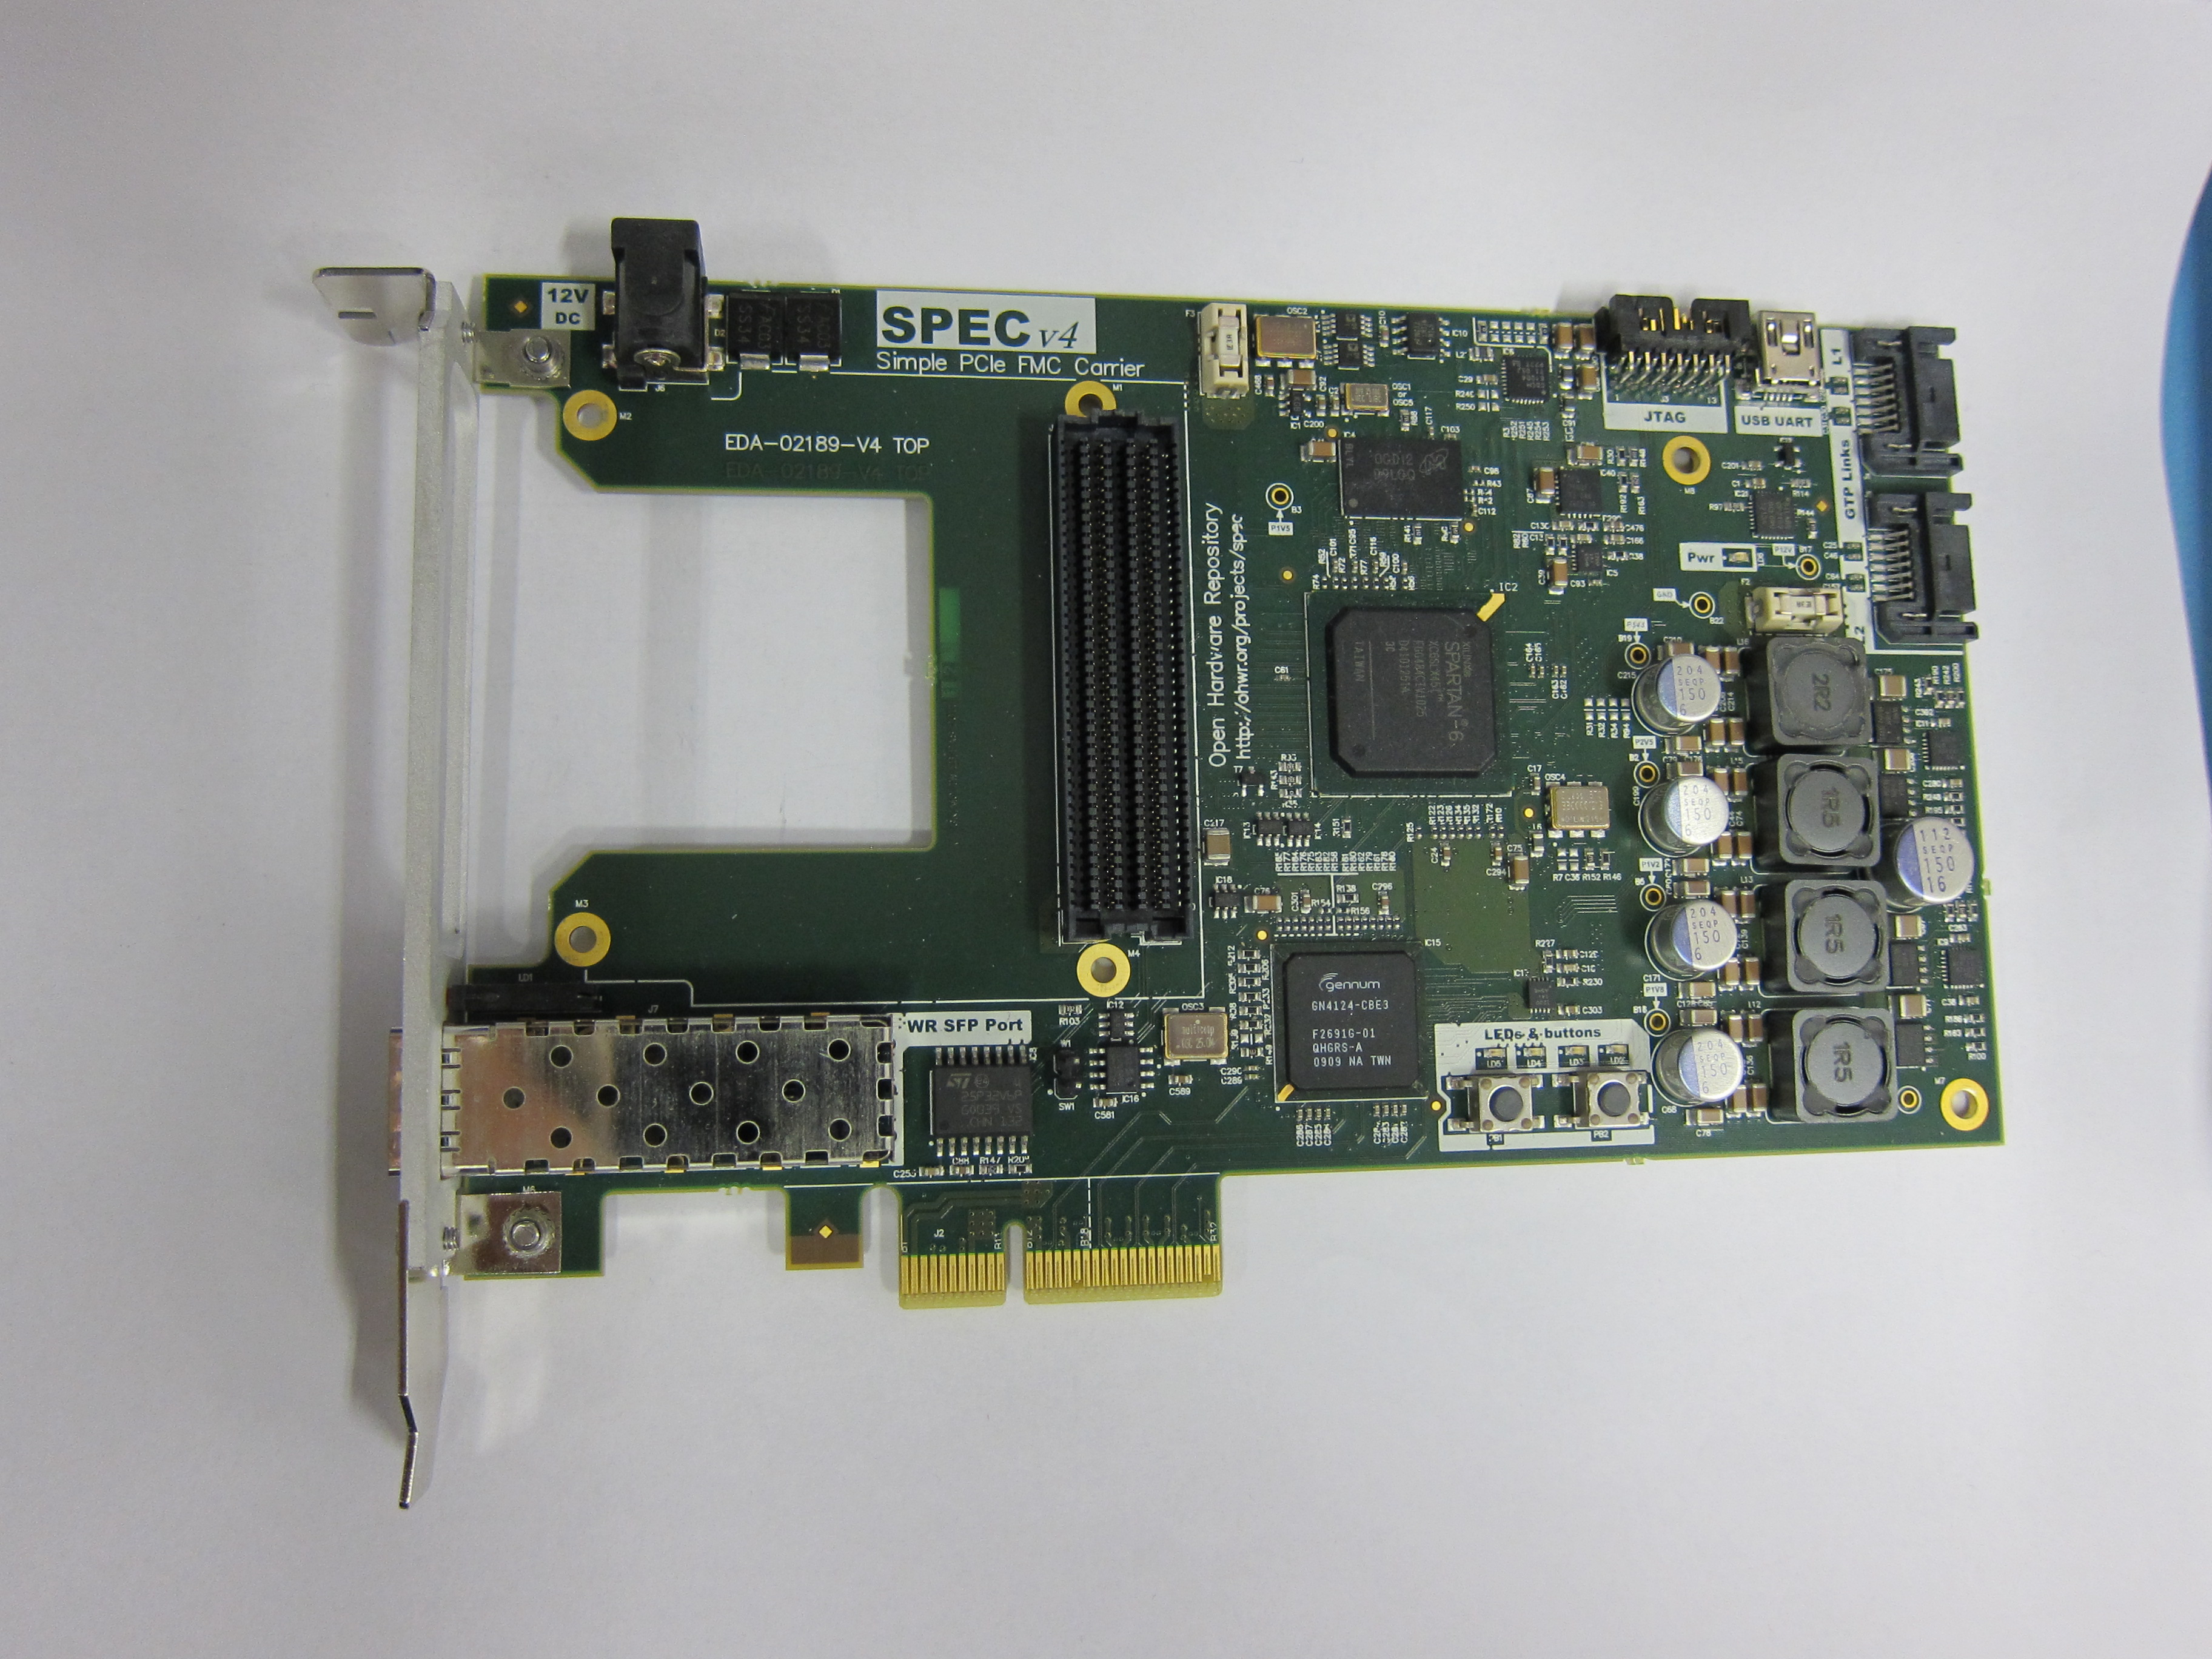
\includegraphics[height=7cm]{../pictures/spec_v4.eps}
  \end{center}

  \note[item]{}

\end{frame}

%------------ FRAME --------------------------------------------------
\begin{frame}{SVEC - Simple VME FMC Carrier}{Commercialised in Germany}

  \begin{center}
    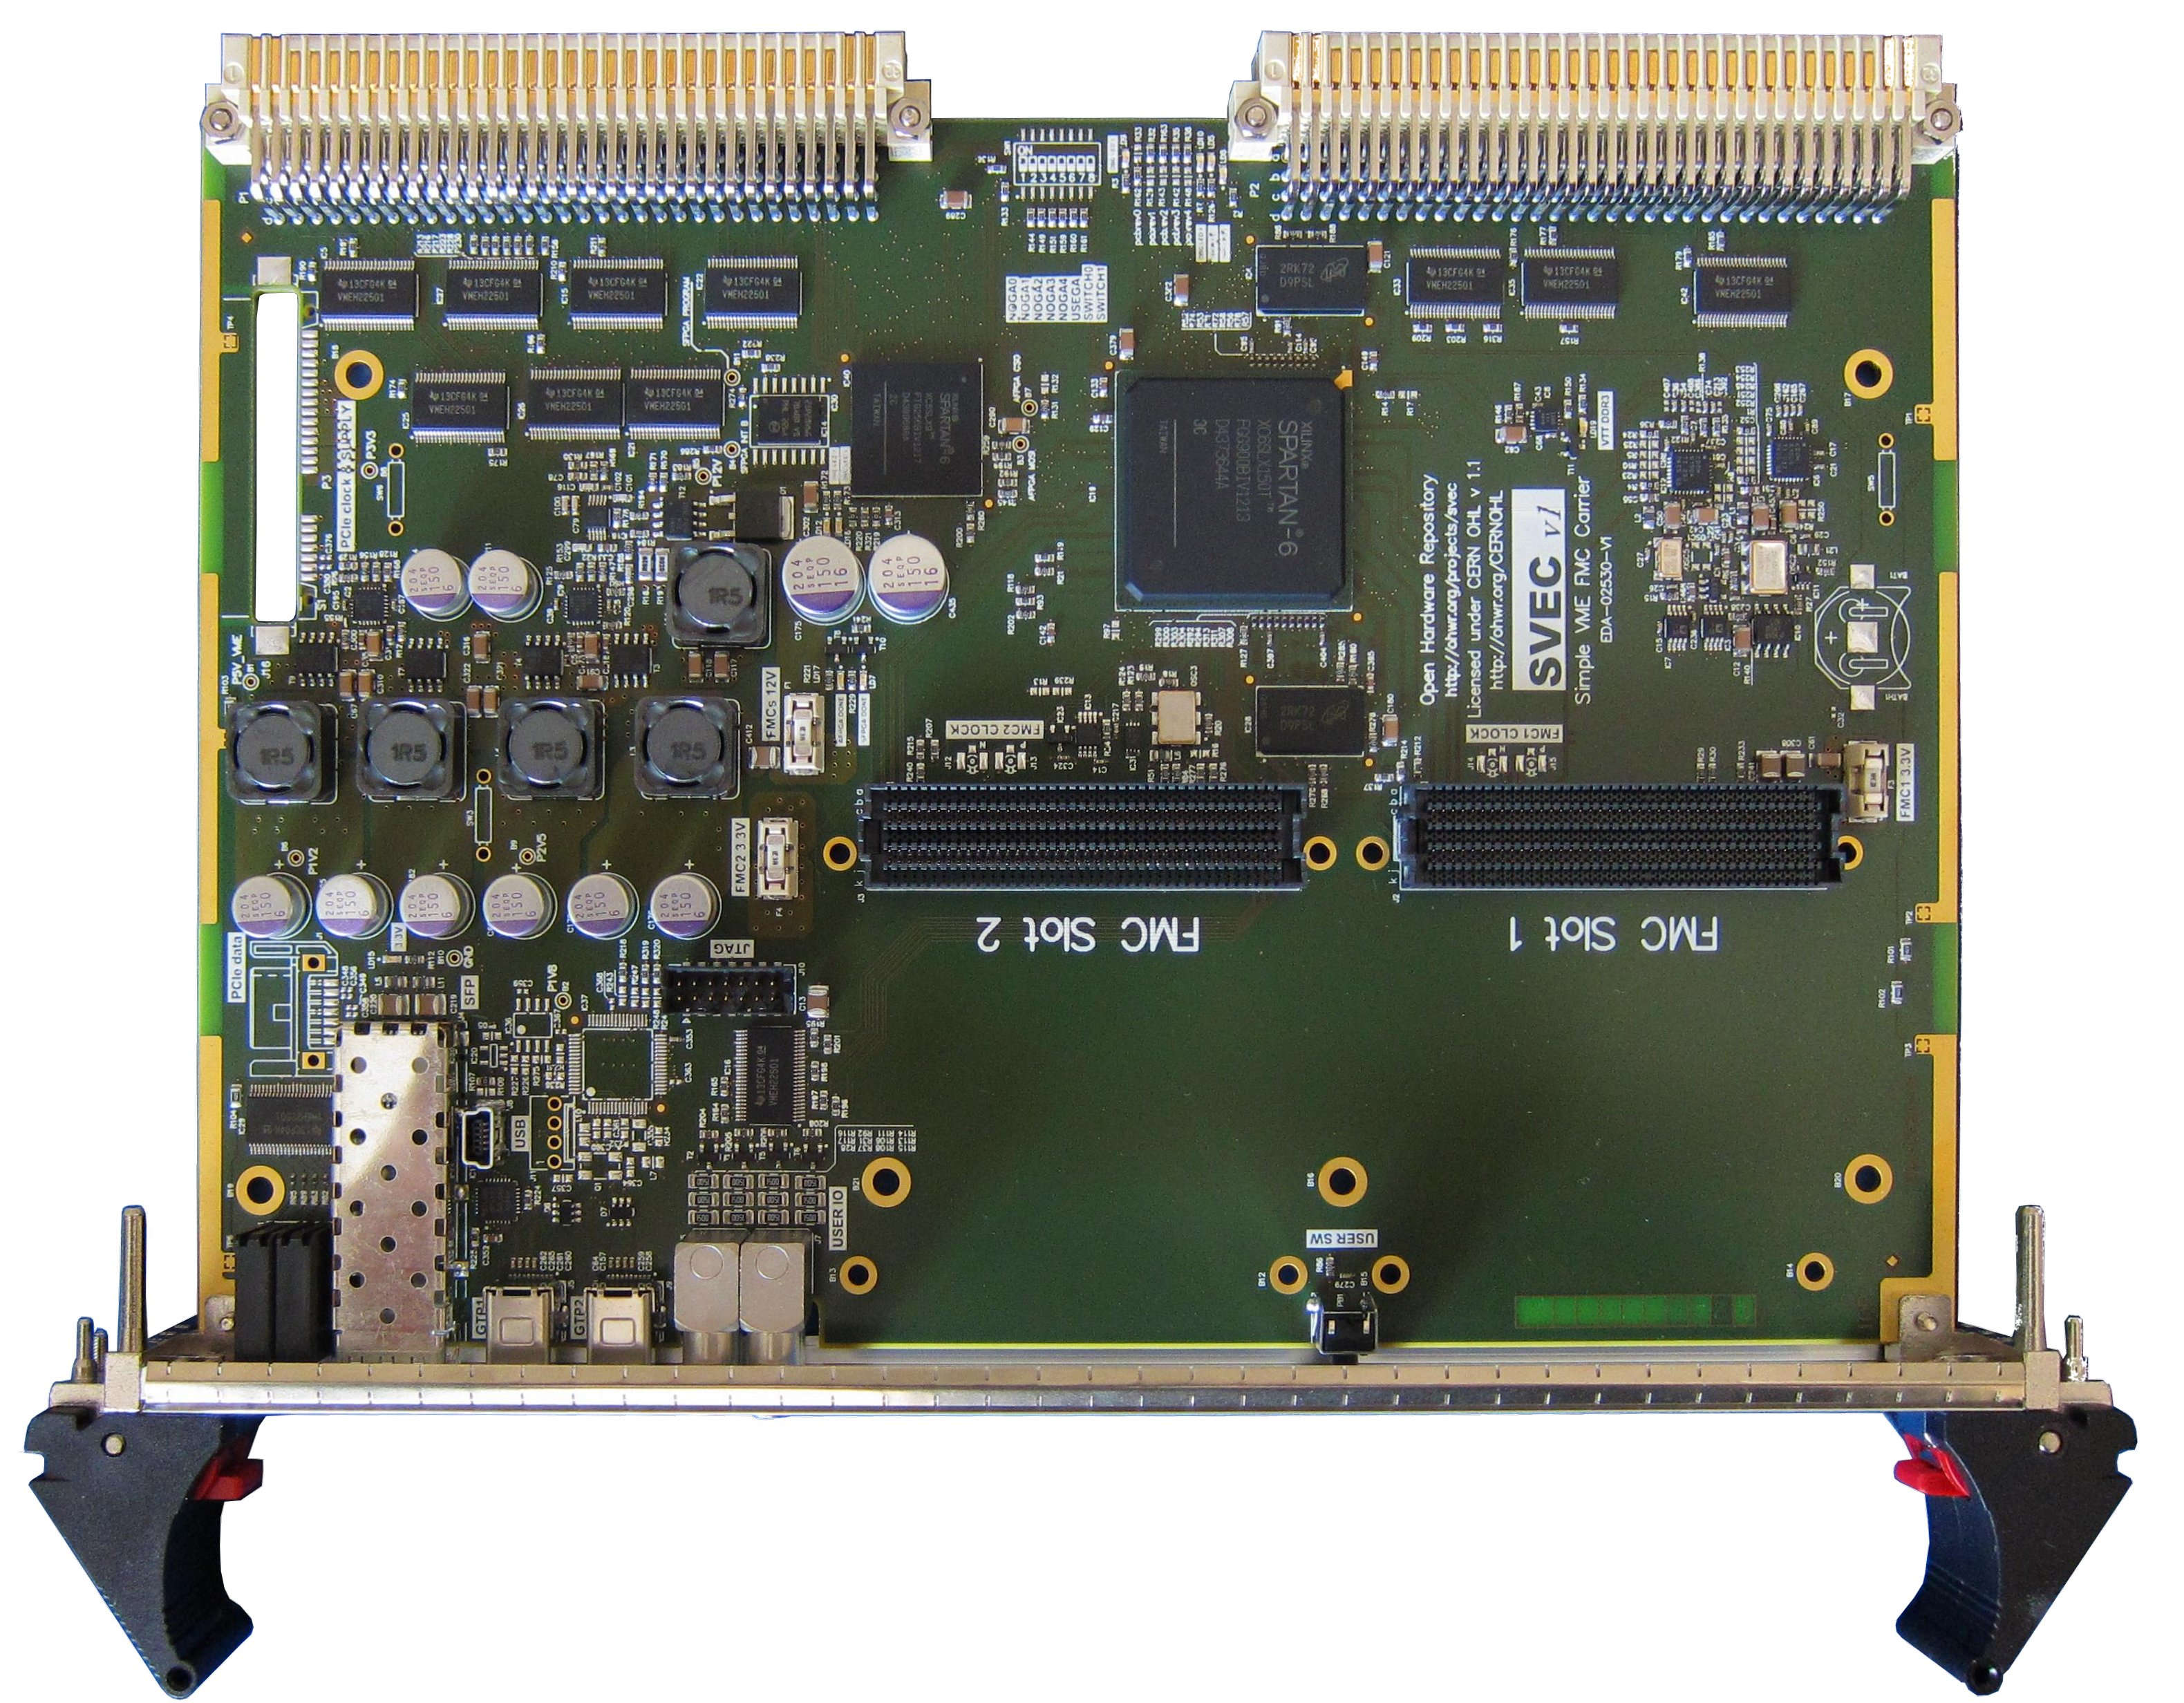
\includegraphics[height=7cm]{../pictures/svec.eps}
  \end{center}

  \note[item]{}

\end{frame}

%------------ FRAME --------------------------------------------------
\begin{frame}{SPEXI - Simple PXI Express FMC carrier}{A modified SPEC board}

  \begin{center}
    \includegraphics[height=7cm]{../pictures/spexi_v0.eps}
  \end{center}

  \note[item]{}

\end{frame}

%------------ FRAME --------------------------------------------------
\begin{frame}{FMC mezzanine: 5-channel 1ns TDC}{A joint development by TE/ABT, TE/CRG \& BE/CO}

  \begin{center}
    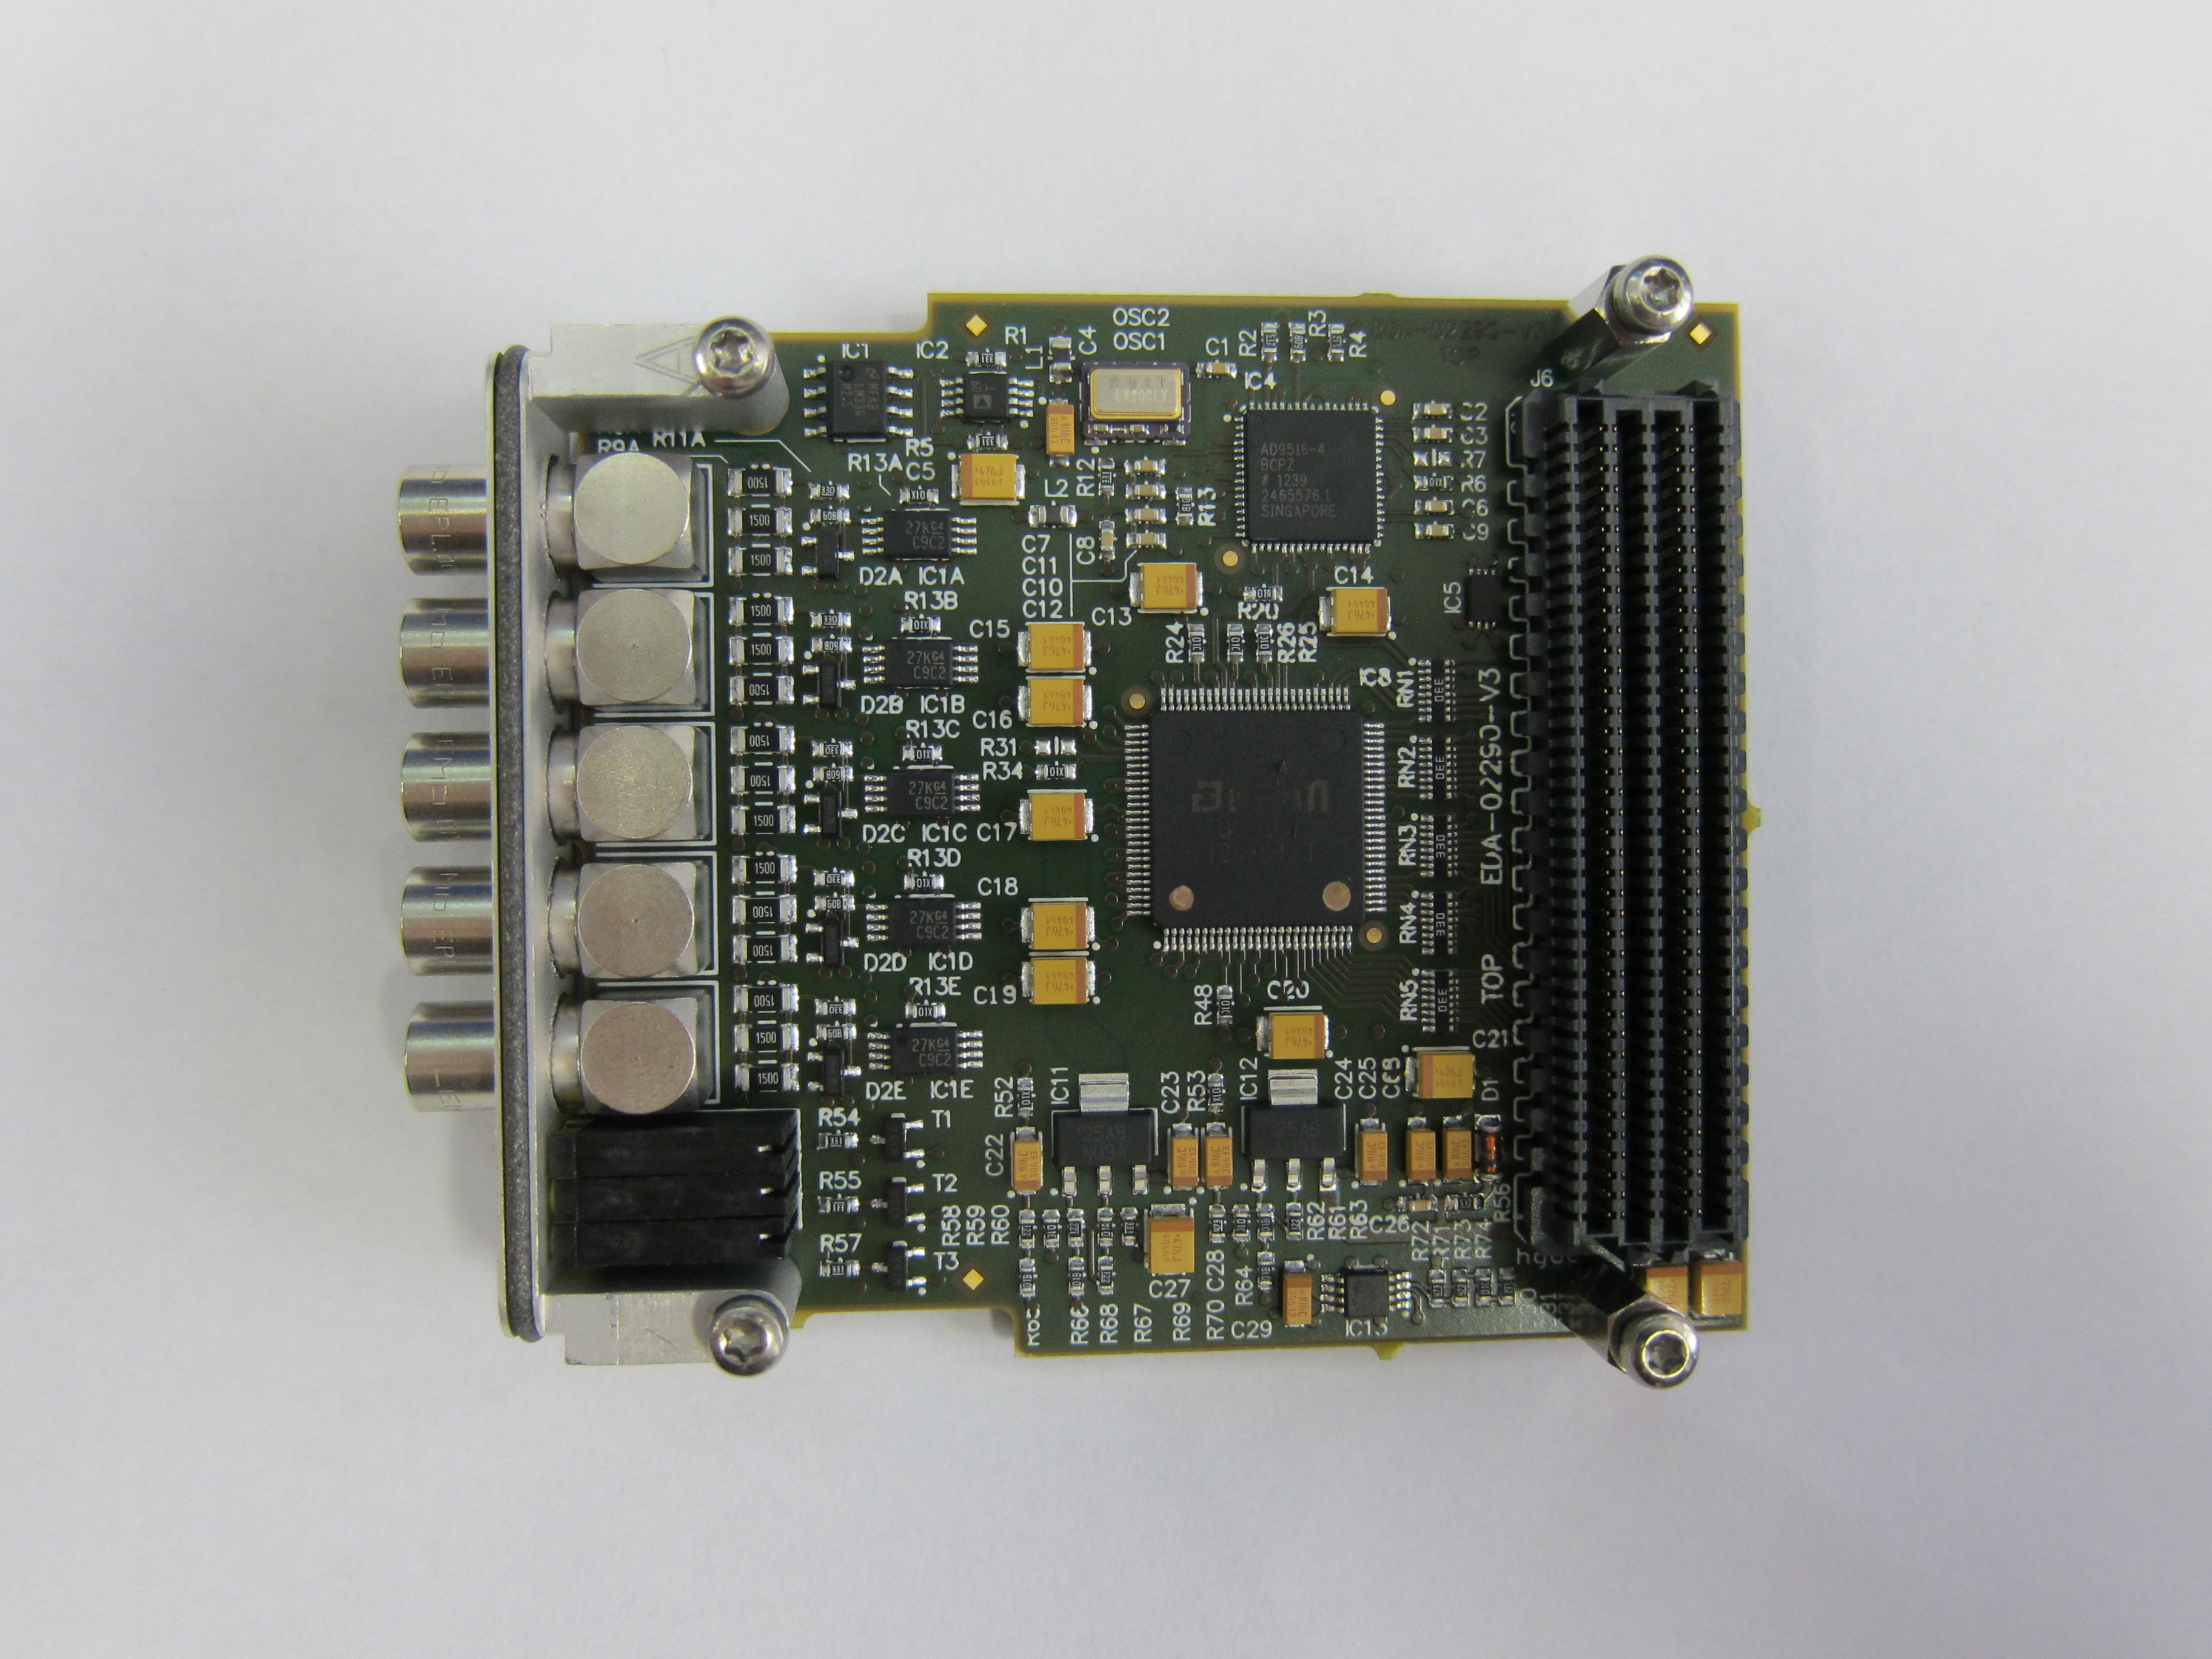
\includegraphics[height=6.5cm]{../pictures/fmc-tdc.eps}
  \end{center}

  \note[item]{}

\end{frame}

%------------ FRAME --------------------------------------------------
\begin{frame}{FMC mezzanine: 100 MSPS 14-bit 4-channel ADC}

  \begin{center}
    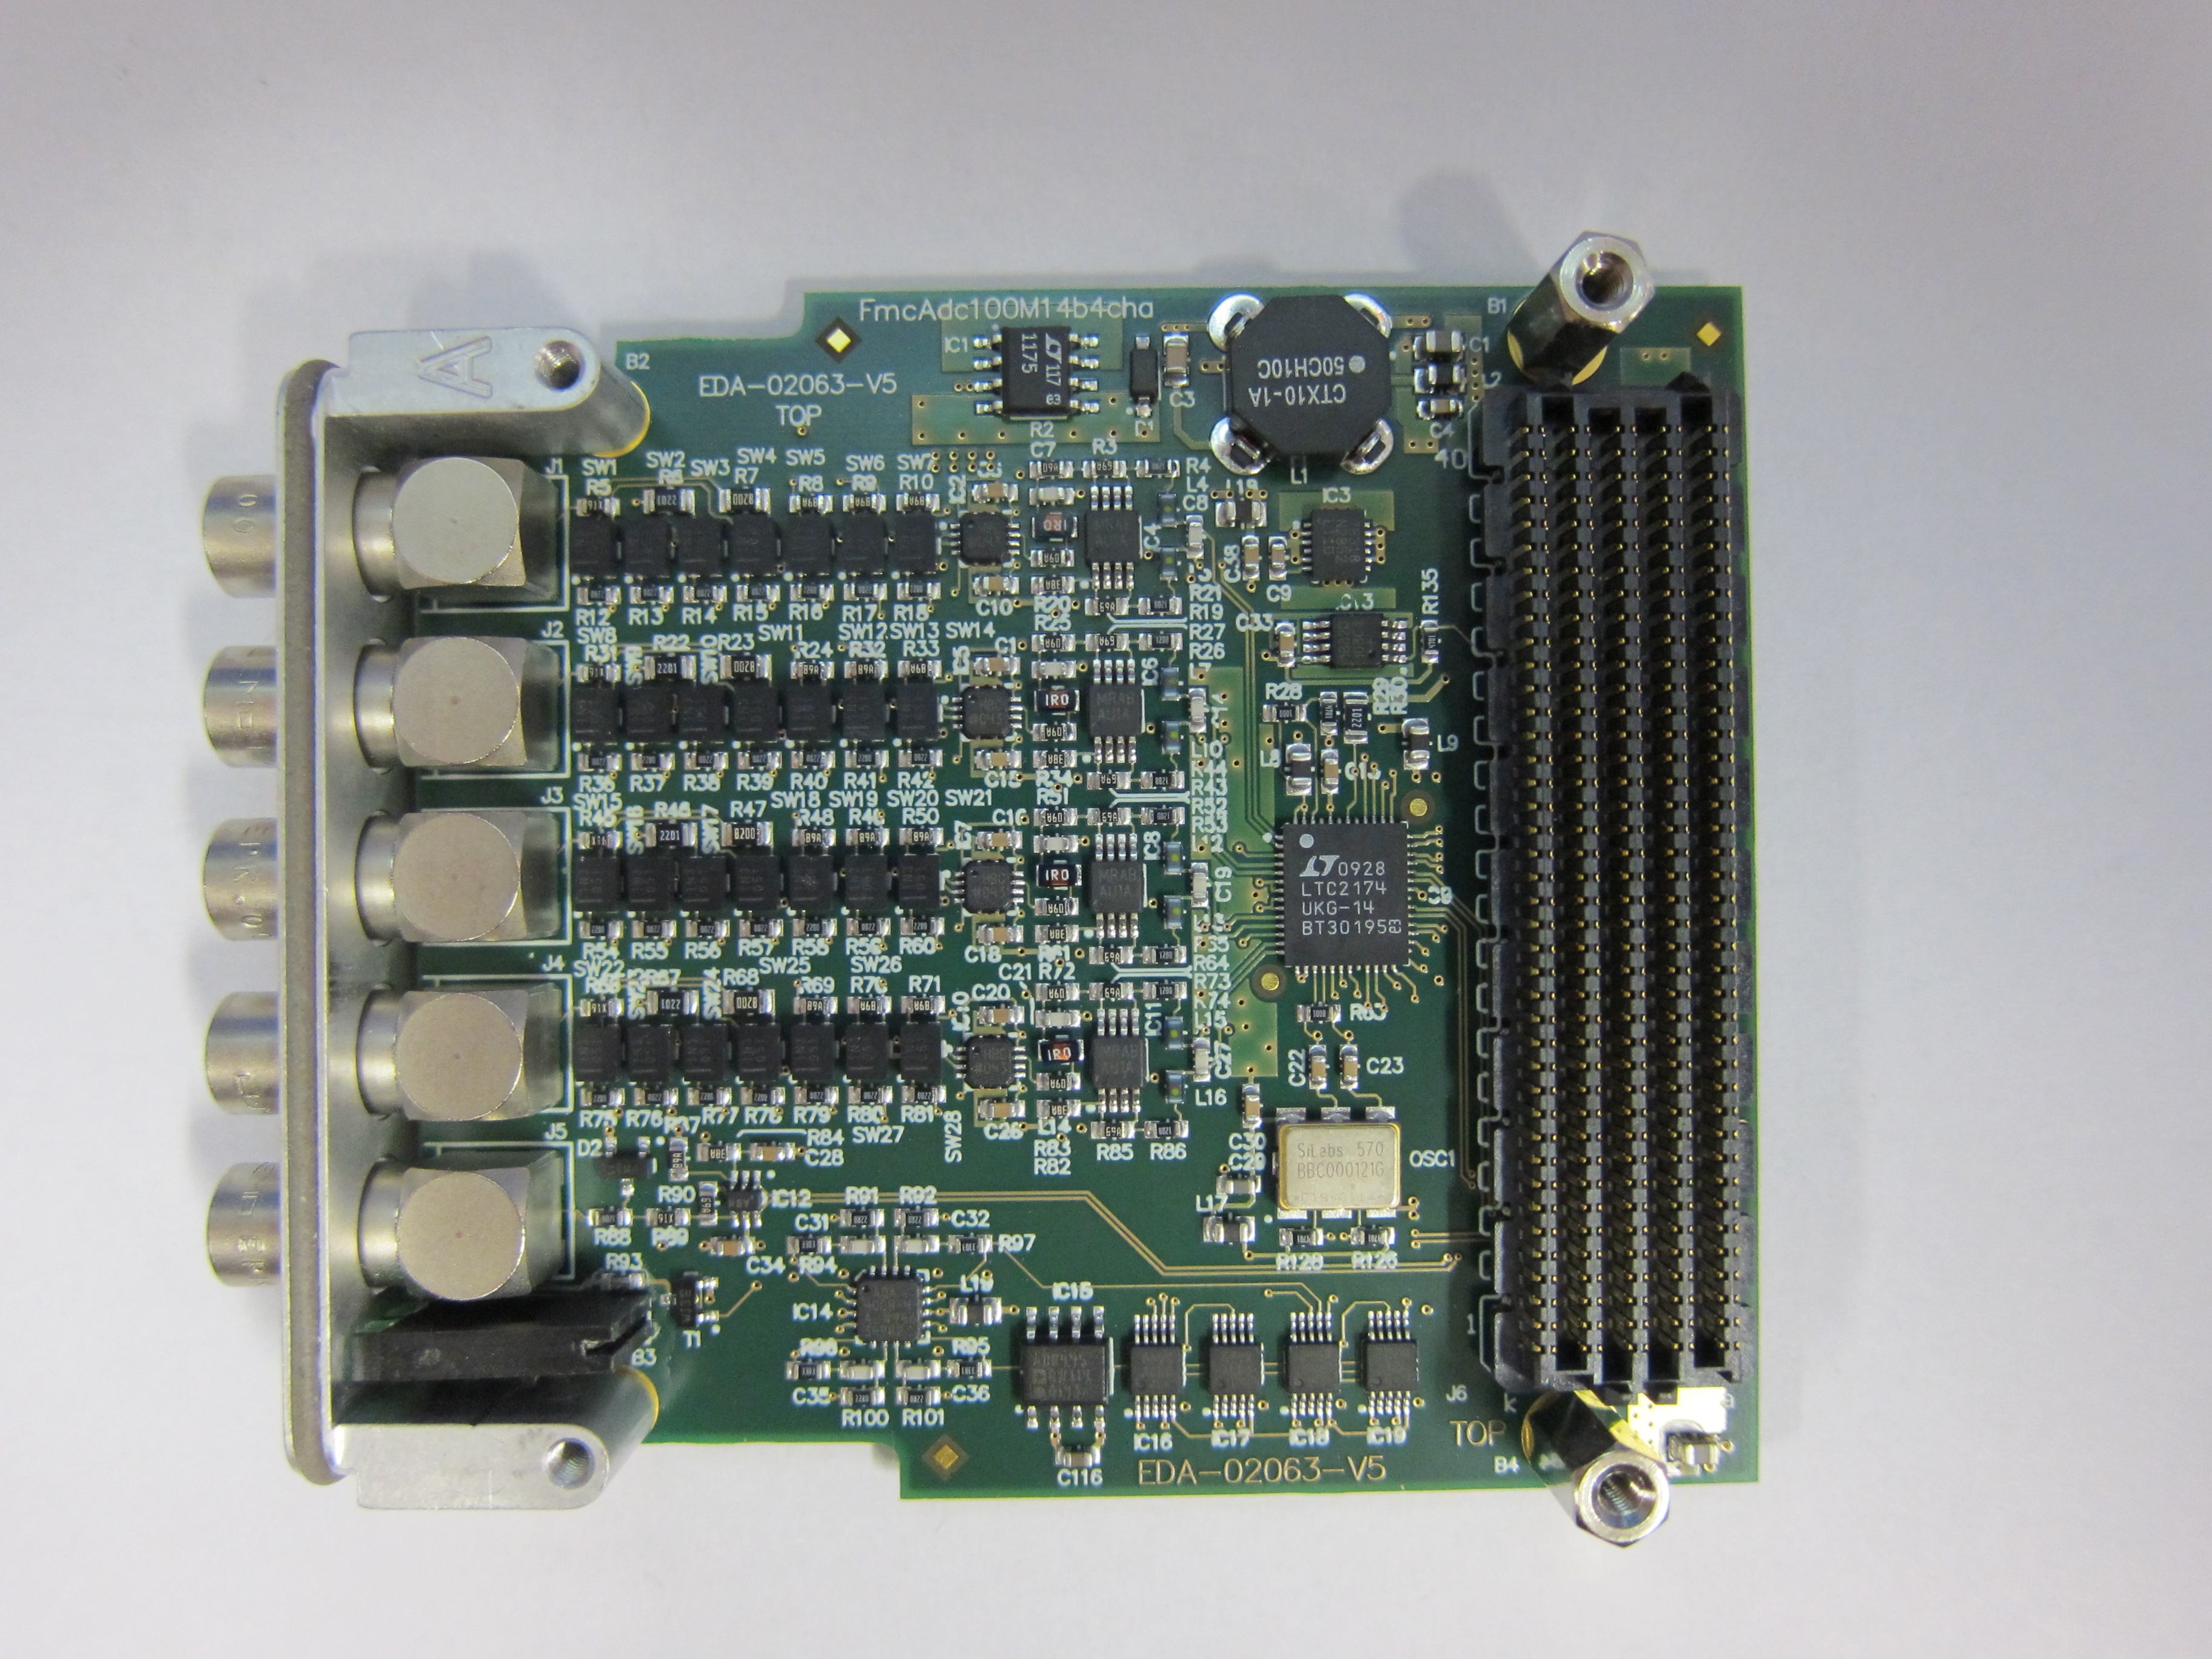
\includegraphics[height=6.5cm]{../pictures/fmc-adc-100m.eps}
  \end{center}

  \note[item]{}

\end{frame}

%------------ FRAME --------------------------------------------------
\begin{frame}{Commercially available CERN OH designs}{September 2013}

  \begin{table}
    \centering

% \begin{tabular}{|l||r|r|r|c|}
    \begin{tabular}{|l||r|r|r|}
      \hline
      Project & Producers & Users & Produced\\
      \hline\hline
      SPEC carrier - PCIe & 3 & 41 & 300 \\
      \hline
      SVEC carrier - VME & 2 & 4 & 105 \\
      \hline
      SPEXI carrier - PXIe & 1 & 2 & (proto) 3 \\
      \hline
      \hline
      ADC 100M 14b 4ch & 2 & 11 & 70 \\
      \hline
      TDC 1ns 5cha & 1 & 3 & 70 \\
      \hline
      FMC DEL 1ns 4cha & 3 & 4 & 108 \\
      \hline
      FMC DIO 5ch & 3 & 10 & 92 \\
      \hline
      \hline
      \textit{WR switch 18 ports} & 1 & 11 & 77\\
      \hline
    \end{tabular}

    \caption{eight CERN OH designs found producers and users}
  \end{table}

  \note[item]{}

\end{frame}


%============ SUB-SECTION ============================================
\section{Gateware architecture}

\subsection*{} % dummy subsection to display dots

%------------ FRAME --------------------------------------------------
\begin{frame}{Gateware architecture}

  \begin{block}{Wishbone for modularity}
    \begin{itemize}
    \item Open standard
    \item Simple, uses few FPGA ressources
    \item Collection of cores already available (OpenCores)
    \end{itemize}
  \end{block}

  \begin{block}{Architecture}
    \begin{itemize}
    \item One or more Wishbone buses
    \item A Wishbone interface on all blocks
    \item Crossbar to interconnect/arbitrate masters and slaves % devlopped in GSI
    \item Design of new cores: VME64x, PCIe, DDR3
    \end{itemize}
  \end{block}

  \note[item]{}

\end{frame}

%------------ FRAME --------------------------------------------------
\begin{frame}{Example: FMC-ADC gateware architecture}

  \begin{center}
    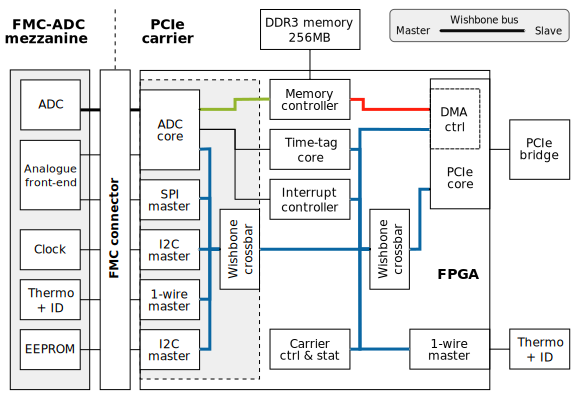
\includegraphics[height=6cm]{../pictures/spec-fmc-adc_arch_simple_color.eps}
  \end{center}

  \note[item]{}

\end{frame}

%============ SUB-SECTION ============================================
\section{Tools and concepts}

\subsection*{} % dummy subsection to display dots

%------------ FRAME --------------------------------------------------
\begin{frame}{Gateware design tools}

  \begin{block}{hdlmake}
    \begin{itemize}
    \item Project structure described in \textit{Manifest} files
    \item Solves dependencies (fetches remote ones)
    \item Generates \textit{Makefile} for synthesis and simulation
    \end{itemize}
  \end{block}

  \begin{block}{wbgen2: Wishbone slave generator}
    \begin{itemize}
    \item Generate register, RAM, FIFO, interrupt controller
    \item Structure described in a single text file
    \item HDL, C header and documentation automatically generated
    \end{itemize}
  \end{block}

  \note[item]{}

\end{frame}

%------------ FRAME --------------------------------------------------
\begin{frame}{wbgen2: HTML documentation example}

  \begin{center}
    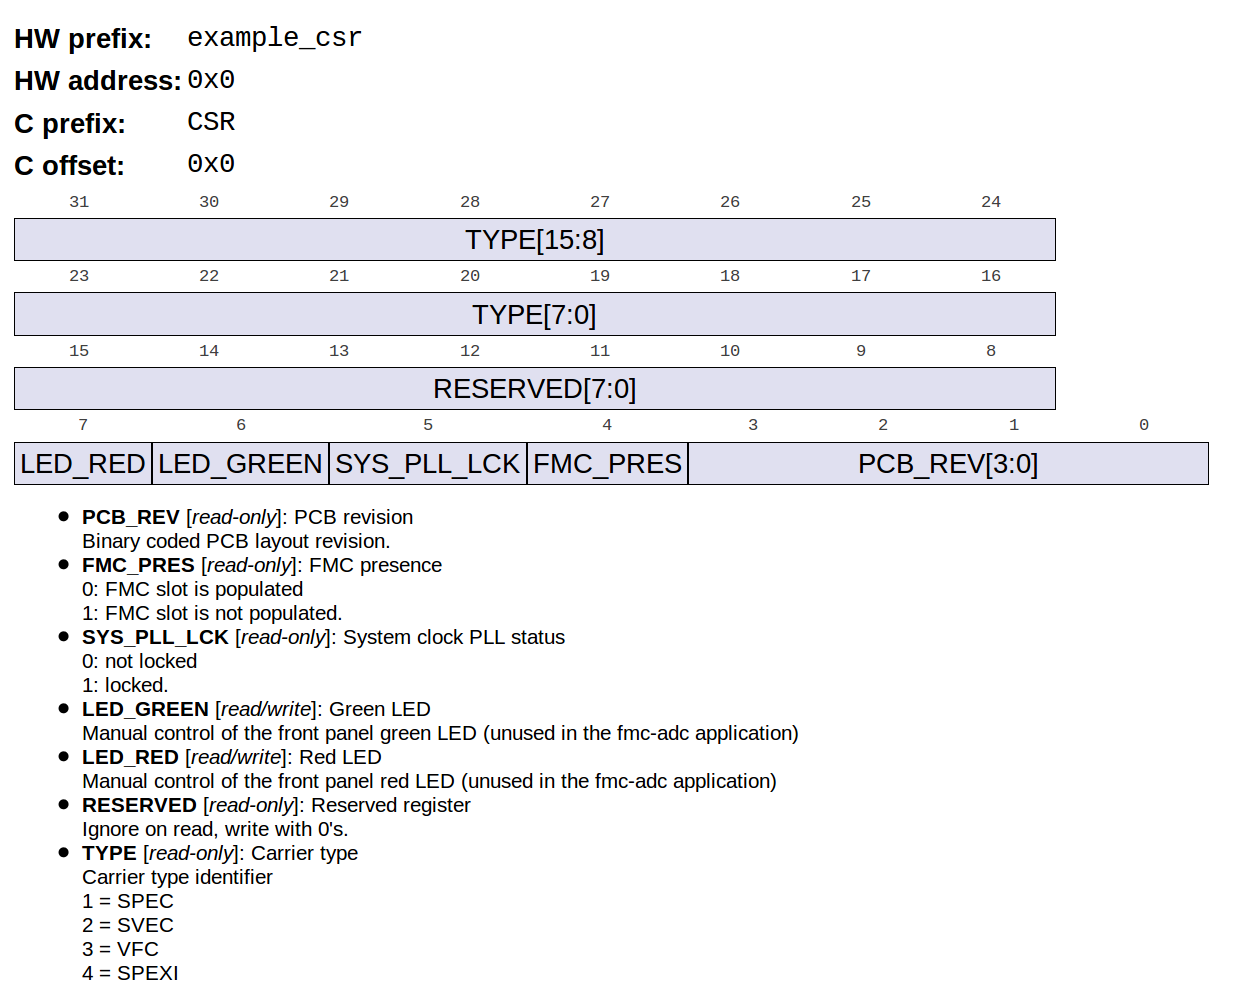
\includegraphics[height=7cm]{../pictures/wbgen_example.eps}
  \end{center}

  \note[item]{This is a example of HTML documentation generated be wbgen2.}

\end{frame}

%------------ FRAME --------------------------------------------------
\begin{frame}{Testing environment}

  \begin{block}{PTS: Production Test Suite}
    \begin{itemize}
    \item Functional test only
    \item Dedicated test setup per board
    \item Software framework to run the tests (Python)
    \item Calibration data stored in FMC EEPROM
    \item Log files (life-cycle management)
    \end{itemize}
  \end{block}

% Before CERN was testing boards
% -> unloads CERN team

% Warranty, repair of faulty boards

  \note[item]{}

\end{frame}

%------------ FRAME --------------------------------------------------
\begin{frame}{Example: VME boards test system}

  \begin{center}
    \includegraphics[height=6.5cm]{../pictures/pts_rack.eps}
  \end{center}

  \note[item]{}

\end{frame}

%------------ FRAME --------------------------------------------------
\begin{frame}{New concepts}

  \begin{block}{SDB: Self Describing Bus}
    \begin{itemize}
    \item Series of predefined structures
    \item Meta-data about cores
    \item Allows software to know about gateware architecture
    \end{itemize}
  \end{block}

  \begin{block}{SDB File System}
    \begin{itemize}
    \item Based on SDB data structures
    \item Easy to parse (e.g. for embedded processor)
    \item Library and tools available % (generate, read)
    \item Used in the FMC EEPROM
    \end{itemize}
  \end{block}

  \note[item]{}

\end{frame}

%------------ FRAME --------------------------------------------------
\begin{frame}{Example: SDB records in Wishbone crossbar}

  \begin{center}
    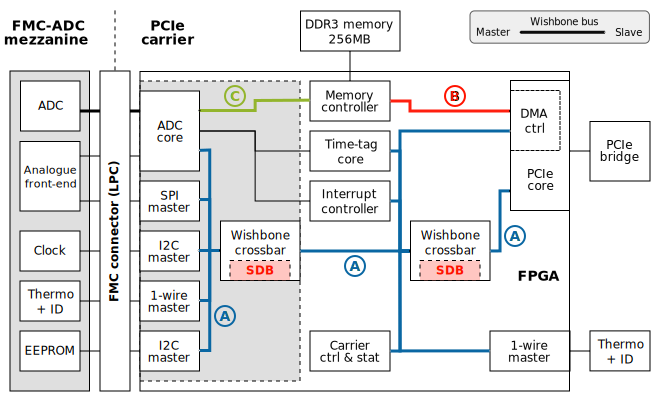
\includegraphics[height=6cm]{../pictures/spec-fmc-adc_arch_simple_color_sdb.eps}
  \end{center}

  \note[item]{}

\end{frame}

%------------ FRAME --------------------------------------------------
\begin{frame}[fragile]{Example: SDB record (VHDL)} % for the workshop

  \small
    \begin{verbatim}
      constant c_ONEWIRE_SDB_DEVICE : t_sdb_device := (
         abi_class     => x"0000",
         abi_ver_major => x"01",
         abi_ver_minor => x"01",
         wbd_endian    => c_sdb_endian_big,
         wbd_width     => x"4",
         sdb_component => (
         addr_first  => x"0000000000000000",
         addr_last   => x"0000000000000007",
         product     => (
            vendor_id => x"000000000000CE42",
            device_id => x"00000602",
            version   => x"00000001",
            date      => x"20121116",
            name      => "WB-Onewire.Control ")));
    \end{verbatim}
    \normalsize

    \note[item]{}

\end{frame}



\begin{comment}
%------------ FRAME --------------------------------------------------
\begin{frame}{FMC EEPROM structure}

  \begin{center}
    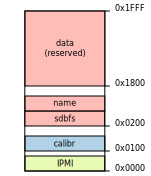
\includegraphics[height=6.5cm]{../pictures/eeprom_struct.eps}
  \end{center}

\end{frame}

% explain fpga fw load (golden -> read eeprom -> final bitstream)

%------------ FRAME --------------------------------------------------
\begin{frame}{Modularity advantages}

  \begin{block}{Easy porting}
    \begin{itemize}
    \item ADC-100M on SPEC = few months
    \item 2x ADC-100M on SVEC = one week
    \end{itemize}
  \end{block}

\end{frame}
\end{comment}



%#####################################################################
%############ SECTION ################################################
\section{Perspectives}

\subsection*{} % dummy subsection to display dots

%------------ FRAME --------------------------------------------------
\begin{frame}{Future work}

  \begin{block}{Consolidate our designs}
    \begin{itemize}
    \item Consolidate gateware and drivers. Make more releases.
    \item Consolidate documentation (manuals, FAQs, ...).
    \item Help companies to provide support.
%    \item Cleanup and unify repositories.
    \end{itemize}
  \end{block}

  \begin{block}{Facilitate sharing with FOSS EDA tools}
    % FOSS = Free Open Source Software, EDA = Electronic Design Automation
    \begin{itemize}
    \item Tools are expensive and do not interoperate.
    \item Existing FOSS tools not usable for complex designs.
    \item We contribute to the development of FOSS tools:
      \begin{itemize}
      \item Extension of \textbf{Icarus} Verilog simulator with VHDL and SV support. % SV = SystemVerilog
      \item Enhancement of \textbf{KiCAD} (schematics \& PCB editor).
      \end{itemize}
    \end{itemize}
  \end{block}

  \note[item]{}

\end{frame}



\begin{comment}
%------------ FRAME --------------------------------------------------
\begin{frame}{New front-end computer platform} % Might skip this slide completly if too long

  \begin{block}{Current platforms limitations}
    \begin{itemize}
%    \item VME64xA
%    \item PICMG 1.3 (PCI and PCIe)
%    \item PXI Express (supported by EN/ICE)
    \item Difficult maintainance (PCI, PCIe)
    \item Low bus throughput (VME, PCI)
    \item No clock and trigger line on backplanes (VME, PCI, PCIe)
    \end{itemize}
  \end{block}

   \begin{block}{Future platform not yet know}
    \begin{itemize}
    \item Just designing a carrier.
    \item Re-useable mezzanines set.
    \item HDL and software framework ready.
    \end{itemize}
  \end{block}

   \note[item]{}

\end{frame}
\end{comment}



%############ SECTION ################################################
\section{Conclusions}

\subsection*{} % dummy subsection to display dots

%------------ FRAME --------------------------------------------------
\begin{frame}{Conclusions}

  \begin{block}{}
    \begin{itemize}
    \item CERN's FMC kit is not only a set of hardware modules
      \begin{itemize}
      \item Collection of HDL cores
      \item Linux device driver and test program
      \item Production test system
      \item Tools and concepts %(wbgen, hdlmake, )
      \item Commercially available (sometimes from several sources)
      \end{itemize}
    \item Open Hardware has many advantages.
      \begin{itemize}
      \item Anyone can help in developments and make improvements.
      \item Allows to work differently with industry. % (design work, smaller companies).
      \item Not tied to a single company for production and support.
      \end{itemize}
    \item Using standards attracts users and improves re-usability. %(VME64x, PCIe, FMC, Wishbone)
    \item OHR site is practical for engineers and is stimulating.
%    \item OHR site contains many re-usable HDL cores.
    \item Good FOSS tools needed to facilitate sharing.
%    \item Many designs being developed and several are already produced by industry.
    \item Four years of experience show it works!
    \end{itemize}
  \end{block}

  \note[item]{}

\end{frame}



\begin{comment}

\begin{frame}{Erik's for TWEPP}

  \begin{itemize}
  \item Open Hardware has many advantages.
    \begin{itemize}
    \item Anyone can help in developments and make improvements.
    \item Allows to work differently with industry (design work, smaller companies).
    \item Not tied to a single company for production and support.
    \end{itemize}
  \item Many things must be done right:
    \begin{itemize}
    \item Be Open
    \item Make design general enough
    \item Use standards - cool features help: White Rabbit
    \item Be complete: from design to production test and drivers
    \item Work intensively with industry
    \end{itemize}
  \item Likely not for everyone or all designs.
  \item OHR site is practical for engineers and is stimulating.
  \item Eight CERN designs are already commercialized.
  \item Four years of experience show it works!
  \end{itemize}

\end{frame}

\begin{frame}{Javier's for OKcon}

  \begin{itemize}
  \item The electronics that we support cannot be black boxes.
  \item Open Hardware has many advantages.
    \begin{itemize}
    \item Anyone can help in developments and make improvements.
    \item Allows to work differently with industry (design work, smaller companies).
    \item Not tied to a single company for production and support.
    \end{itemize}
  \item {CERN Open Hardware License} provides a legal basis.
    %\item Using standards (VME64x, PCIe, FMC, Wishbone) attracts users and improves re-usability.w
  \item OHR site is practical, stimulating and fun for engineers.
    %\item OHR site contains many re-usable HDL cores.
  \item Good FOSS tools needed: help us make it happen!
  \item Many designs being developed and several are already produced by industry.
  \item Four years of experience show it works!
  \end{itemize}

\end{frame}

\end{comment}

%------------ FRAME --------------------------------------------------
% Erik's slide with products webpages?



%\vspace{0.2cm}
%Opening up your designs does make you more vulnerable to this disease.
%\end{frame}
%%One slide to justify our license choice so far
%% One slide on evil patents and the risk for open design.

\end{document}


